\usepackage[nohead, textwidth=16.5cm, textheight=23.5cm, ignorehead, paper=a4paper]{geometry}
\usepackage{fontspec}
\usepackage{graphicx}
\usepackage[french]{babel}
\usepackage{hyperref}
\usepackage{tikz}
%\usepackage{parskip}
\usepackage{enumitem}
\usepackage{url}
\usepackage{tabulary}
\usepackage{enumitem}
\usepackage{titlesec}
\usepackage{titletoc}
\usepackage{etoolbox}
\usepackage{intcalc}
\usepackage[absolute]{textpos}

\newcommand{\pvfred}{40\ieme{}}
\newcommand{\pvfryear}{2017}
\newcommand{\pvfrstartfr}{10 juillet}
\newcommand{\pvfrendfr}{6 août}
\newcommand{\pvfrstartde}{10. Juli}
\newcommand{\pvfrendde}{6. August}


\AtBeginDocument{\def\labelitemi{$\bullet$}}

\setmainfont{Alegreya Sans}
\setkomafont{disposition}{\normalfont}
% \setcounter{tocdepth}{1}

\renewcommand{\leftmark}{}
\renewcommand{\rightmark}{}

\hypersetup{
    pdftitle={Passeport vacances Fribourg \pvfryear},
    pdfauthor={Jacques Supcik},
    bookmarks=true,
}

\begin{document}
\frontmatter
\begin{titlepage}
\begin{center}
{\fontsize{45}{40}\selectfont{}\pvfred{} Passeport vacances\\
\vspace*{3mm}
Fribourg/Freiburg \pvfryear}
\vfill
\includegraphics[width=.7\textwidth]{fig/logo.jpg}
\vfill
{\fontsize{32}{32}\selectfont{}du \pvfrstartfr{} au \pvfrendfr{} \pvfryear}\\
\vspace*{3mm}
{\fontsize{32}{32}\selectfont{}vom \pvfrstartde{} bis \pvfrendde{} \pvfryear}

\end{center}
\end{titlepage}
\ifbare
\else
\clearpage
\cleardoublepage
Nous avons fait tout notre possible pour que le 39ème programme du Passeport vacances Fribourg vous plaise et vous souhaitons de bonnes vacances!
	
\textbf{Ont participé à l'élaboration du programme:}

\begin{tabular}{p{1.6cm} l}
Mmes & Claudine Audriaz \\
& Patricia Dupont \\
& Nathalie Marvardi-Bürgy \\
\end{tabular}

\begin{tabular}{p{1.6cm} l}
	MM. & Hubert Audriaz \\
	& Jocelyn Audriaz \\
	& Dominique Dupont \\
	& Laurent Kolly \\
	& Jacques Supcik \\
\end{tabular}

Avec la collaboration de personnes assignées par le SIAS de la Ville de Fribourg (PET via le SPE et contrats auxiliaires via OCOT). 

Avec la participation des élèves de l'ECGF (Ecole de Culture Générale de Fribourg) dans le cadre de leur stage obligatoire.




\clearpage%
\thispagestyle{empty}%
\centering{
\includegraphics[width=\textwidth]{pub1.jpg}
\par
}

\fi
\cleardoublepage
\tableofcontents
\cleardoublepage

\mainmatter

\ifbare
\else
\part{Informations générales}
\chapter{Informations}

\section*{Organisateurs}

Passeport vacances Fribourg, ch. du Grabensaal 4, 1700 Fribourg

\section*{Site Internet}

\url{www.passeport-vacances-fribourg.ch}

\section*{Facebook}

\url{https://www.facebook.com/passeportvacancesfribourg}

\section*{Courriel}

\begin{itemize}
\item Secrétariat: \url{passvac.fribourg@bluewin.ch}
\item Contact pour questions générales et de matériel: \url{pass_vac@hotmail.fr}
\end{itemize}

\section*{Age}

Le passeport est destiné aux enfants de 7 à 16 ans.

\section*{Prix et durée du passeport}

Le prix d'un passeport est de 35 francs (sauf dans les rares cas où la Commune
du détenteur ne participe pas financièrement).

Il est valable deux semaines au choix entre le 11 juillet et le 7 août 2016 et
permet de participer à la grande fête finale qui aura lieu le vendredi5 août
2016, également si votre passeport est périmé.

Le passeport du troisième enfant d'une même famille est gratuit, sur
présentation du livret de famille. Dans ce cas, les passeports doivent être
achetés en même temps mais les dates d'utilisation peuvent être différentes.

Le passeport est personnel et les enfants doivent l'avoir sur eux lors de chaque
activité. En cas de perte ou s'il n'est pas utilisé, il n'est pas remboursé.

\section*{Prestations}

Dans le prix du passeport sont compris:

\begin{itemize}
\item un libre accès à l'ensemble du réseau régional et urbain des TPF
\item coupons à utiliser pour …………. et une partie gratuite de minigolf
\item l'entrée gratuite dans 5 musées, aux piscines de la Motta et du Levant et
un accès à la Tour de la Cathédrale Saint-Léonard
\item le prêt de livres et jeux
\item un tour en petit train du Gottéron
\item du hockey et du patinage libre les samedis ………………
\item le concours "………"
\item l'accueil midi.
\end{itemize}

Il comprend également des activités qui nécessitent une inscription sur Internet
(v. point suivant "Comment faire?")

\section*{Comment faire?}
\begin{enumerate}
\item A partir du 2 juin 2016, rendez-vous auprès d'un des quatre lieux de vente
avec une photo et le montant à payer. Il vous sera remis le passeport et la
présente brochure.
\item Du 11 au 25 juin 2016, allez sur le site www………………….. et cliquez sur
"inscriptions".
\begin{itemize}
\item Cliquez maintenant sur la fleur qui vous permet d'accéder à l'adresse
http://groople.me/............
\item Sur cette première page, entrez les coordonnées demandées. Notez à part
votre nom d'utilisateur et votre mot de passe qui vous seront utiles plus
tard. Enregistrez.
\item Pour continuer votre inscription, allez dans votre messagerie. Vous avez
reçu un courriel qui vous demande de bien vouloir confirmer votre
inscription. Cliquez sur le lien qui vous est donné et vous pourrez ainsi
continuer l'inscription et choisir les activités.
\item Sur cette page, tous les jours de la période du Passeport vacances sont
cochés. Décrochez les jours auxquels vous êtes absents. Cliquez sur
continuer.
\item Sur cette page, il y a toutes les activités en rapport à votre âge et votre
disponibilité. Pour avoir plus d'informations sur une activité, cliquez sur le
point d'interrogation. Choisissez maintenant vos activités par ordre de
préférence, en cliquant sur les bulles de couleur. Certaines bulles sont
grises, ce sont les jours où vous êtes absents. Cliquez sur continuer.
\item Vous avez fini votre inscription. Une longue liste de vos choix s'affiche.
Cliquez maintenant sur terminer. Vous pouvez sortir de Groople.
\item Vous recevrez un deuxième courriel avec la confirmation que vos choix ont
bien été enregistrés.
\end{itemize}
\item Le 27 juin 2016, le système attribuera les activités et vous l'enverra par
courriel.
\item Du 29 juin au 3 juillet 2016, une bourse aux places restantes sera mise en
ligne.
\item Les 4 et 5 juillet 2016, vous recevrez par courriel la liste définitive de vos
activités.
\end{enumerate}

\section*{Inscriptions assistées}

Pour ceux qui n'ont pas la possibilité de s'inscrire sur Internet ou qui
rencontrent des problèmes, nous vous donnons rendez-vous à l'Office du
tourisme de Fribourg, place Jean-Tinguely 1 à Fribourg (bâtiment Equilibre) les
samedis 11 et 25 juin de 9h00 à 15h00. Des membres du comité se tiendront à
votre disposition pour vous aider dans le processus d'inscription et répondront
à vos questions.

\section*{Lieux de vente}

\begin{itemize}
\item Office du tourisme de Fribourg, bâtiment Equilibre
\item Secrétariat communal de Givisiez
\item Secrétariat communal de Marly
\item Secrétariat communal de Granges-Paccot
\end{itemize}

\section*{Permanence}

Durant les quatre semaines du Passeport vacances, une permanence
téléphonique est à votre disposition pour tous les renseignements, excuses et
divers. Elle sera à votre écoute au numéro …………….. de …..h à ……..h (Mme
Claudine Audriaz).

\section*{Horaires}

Nous demandons aux participants d'être à l'heure. Les organisateurs ou les
accompagnants ne sont pas tenus d'attendre. Lorsque le bus est utilisé pour se
rendre à une activité, il se peut que l'heure du retour ne soit pas tout à fait
respectée, en raison du trafic sur les routes. Nous vous remercions d'avance
pour votre compréhension.

\section*{Discipline}

Les participants inscrits à une activité doivent y participer. En cas de réel
empêchement, prière d'avertir la permanence ………………. Après chaque
activité, ils remercient l'organisateur.

\section*{Assurances}

Tous les participants doivent être assurés en cas d'accident et sont
responsables des dommages qu'ils pourraient causer. Les organisateurs
déclinent toute responsabilité en cas d'accident.

\section*{Comment nous soutenir ?}

\begin{description}
\item [Par un don]
Chaque don sera apprécié à sa juste valeur (CCP 17-1741-4)
\item [En nous proposant du matériel]
Nous avons toujours besoin de matériel divers pour réaliser et préparer
nos activités. Vous pouvez nous faire des propositions en nous adressant
un courriel à \url{pass\_vac@hotmail.fr}
\item [Par du bénévolat]
Si vous souhaitez participer bénévolement à nos activités pour les
enfants, n’hésitez pas à nous envoyer un courriel à \url{pass_vac@hotmail.fr}
\end{description}
\clearpage
\thispagestyle{empty}%
{\centering
\includegraphics[width=\textwidth]{fig/fripass.jpg}
\par
}
\clearpage
\thispagestyle{empty}%
{\centering
\includegraphics[width=.95\textwidth]{fig/taxi.pdf}
\par
\vspace*{20mm}

{\Huge
Nouveau: Minicar 31 places VIP}
\par
\includegraphics[width=.8\textwidth]{fig/bus.png}
\par
}
\clearpage
\thispagestyle{empty}%
{\centering
\includegraphics[width=\textwidth]{fig/tpf2.jpg}
\par
}
\clearpage
\thispagestyle{empty}%
{\centering

\includegraphics[width=\textwidth]{fig/bcf.jpg}
\par
\vspace*{20mm}
\vfill
\includegraphics[width=.8\textwidth]{fig/ville.pdf}
\vfill
\par
}

\fi

\part{Activités}
\chapter{CAT1}
\section{S1}
Hello
\chapter{CAT2}
\section{S2}
Hello


\ifbare
\else
%\clearpage%
%\ifodd\value{page}\hbox{}\newpage\fi%
\cleardoublepage

\begin{center}
{\Huge Plusieurs activités sont financées par la}
\vspace*{5mm}
\par
\includegraphics[width=0.85\textwidth]{regie_fribourg.pdf}
\end{center}

\vfill
\begin{center}
	{\Huge et}
\end{center}
\vfill

\begin{center}
{\Huge par les comités de la Saint Nicolas\vspace*{1mm}\\
du Collège St-Michel}
\vspace*{5mm}
\par
\includegraphics[width=0.8\textwidth]{csm.jpg}
\end{center}


\clearpage
\thispagestyle{empty}%
\includegraphics[width=\textwidth]{ensemble.jpg}
\clearpage
\section*{Réseau régional\\Stadtnetz Regio}
\begin{textblock}{2}(11,1.3)
\includegraphics[width=3cm]{tpf.pdf}
\end{textblock}
\begin{center}
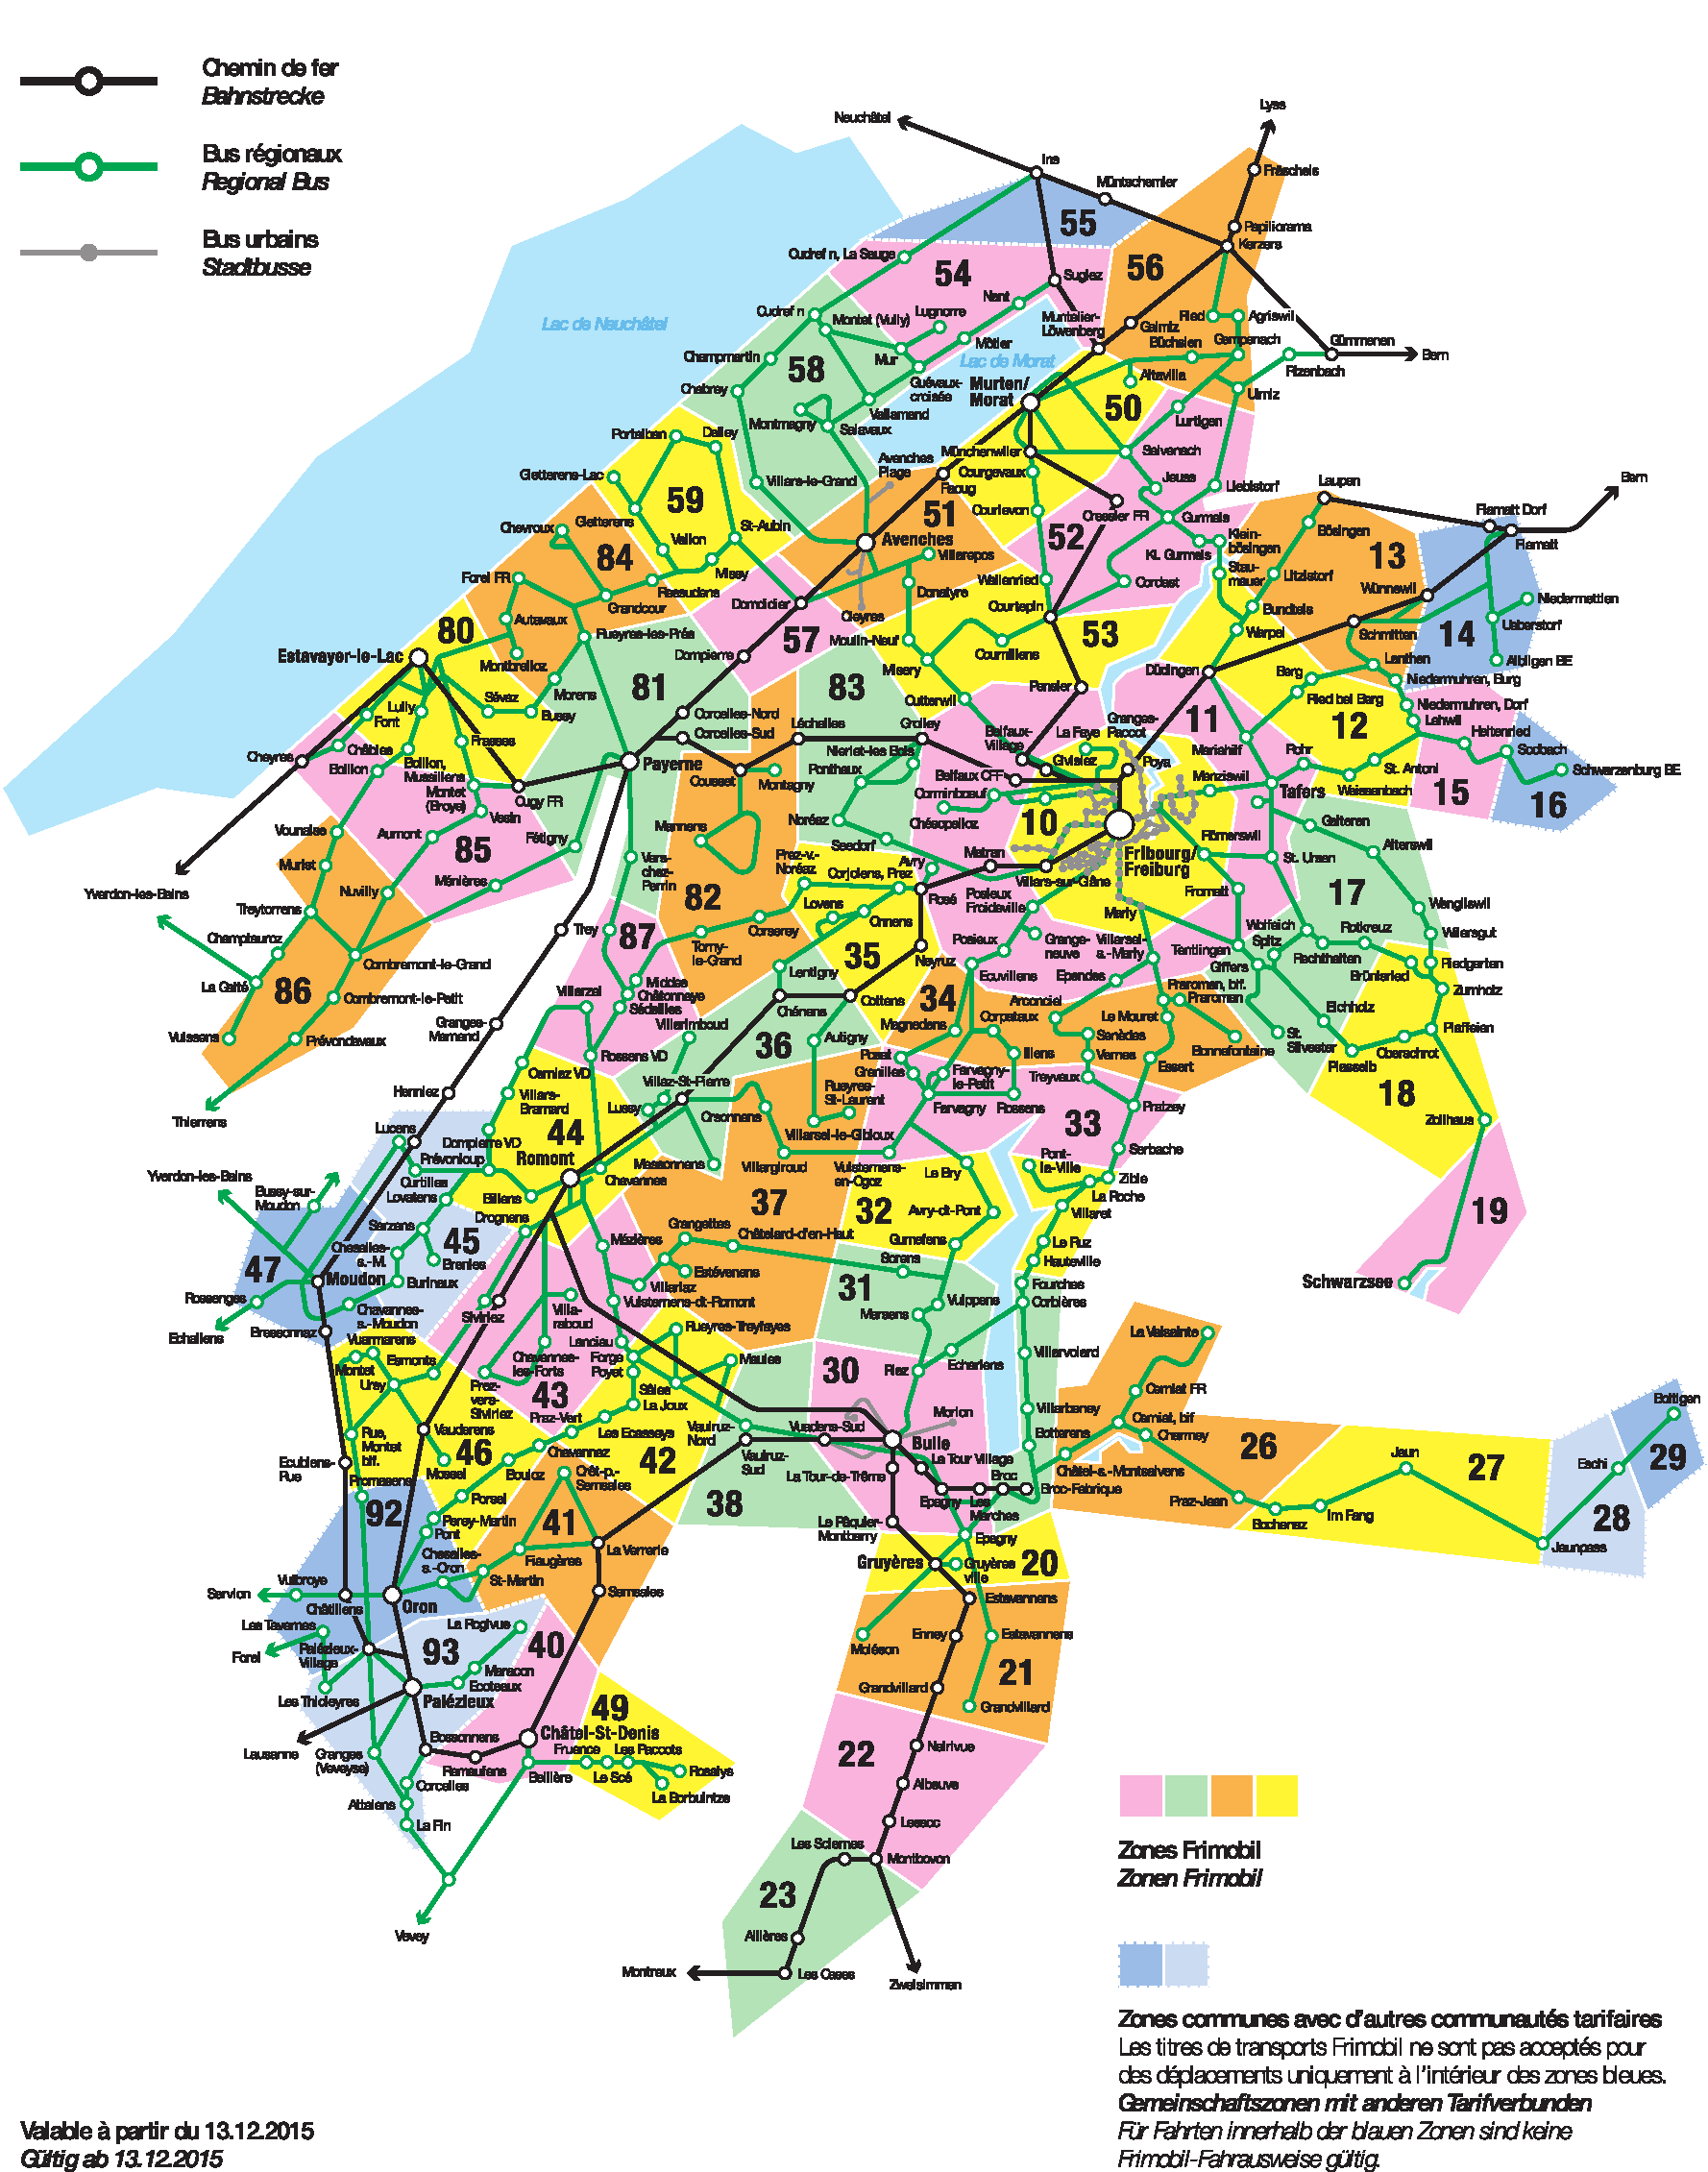
\includegraphics[width=\textwidth]{plan_regional.png}
\end{center}
\clearpage%
\thispagestyle{empty}%
\section*{Réseau Agglo Fribourg\\Stadtnetz Freiburg}%
\begin{textblock}{2}(11,1.3)%
\includegraphics[width=3cm]{tpf.pdf}%
\end{textblock}%
\begin{center}
\includegraphics[width=\textwidth]{plan_zone_10.png}
\end{center}

\fi

\end{document}